% !TEX root=/home/tavant/these/manuscript/src/manuscript.tex

\section{Instability in the \ac{2D} radial-azimuthal \ac{PIC} simulations}
  \label{sec-PIC-ECDI}
  
  \subsection{Introduction and state of the art} \label{subsec-indroECDI}
    
    
    The presence of azimuthal instabilities in the Hall effect thrusters has first been shown with numerical simulations by \citet{adam2004}.
    Then, they have been the subject of numerous studies, especially numerical \citep{ducrocq2006,lafleur2016,lafleur2016a,croes2017,croes2018,janhunen2018,taccogna2019}, but also experimental \citep{honore2011,cavalier2013,cavalier2013a}.
    However, their nature remain unclear \citep{boeuf2018}.

    \vspace{1ex}
    During my PhD, other groups presented their simulation results in a similar radial-azimuthal geometries. They are discussed here.
    
    \citet{hara2019a} presents some kinetic simulation results of a \ac{2D} geometry, of size similar to the case presented here.
    However, the authors focused on the electron mobility values, and few information on the instability are given.
    
    In \citet{janhunen2018}, the authors present a collision-less highly resolved \ac{2D} \ac{PIC} simulation.
    No convection, and no radial losses compensation models are used, hence the electron energy quickly rises and the density decreases.
    On the other hand, the domain is bigger, with a radial length of $L_r = 53.8\,\milli\meter$ for an azimythal length of $L_{\theta} = 13.45 \,\milli\meter$.
    Three cells by Debye length are used, while there are in average 800 particles per cell.
    In these conditions, the instability rises, but a large radial structure, named Modified Two Stream Instability (MTSI), of wavelength twice as big as $L_r$  is observed.
    
    The simulation parameters of \citet{taccogna2019} are similar to the results presented here, with  $L_r = 15\,\milli\meter$ and $L_{\theta} = 12.5 \,\milli\meter$.
    The results are qualitatively similar to the others, however the authors also observed radial structures, but this time with a wavelength of a third of $L_r$.
        
    \vspace{1ex}
    We can see that the results obtained differ, meaning that some points needs to be clarified.
    Thus, we present in this chapter the results obtained with \LPPic.
    
    In \cref{sec-PIC-ECDI}, we present the oscillations observed in the \ac{PIC} simulations.
    After that, we derive the dispersion relation with no hypothesis concerning the particle distribution functions in \cref{sec-DR-kinetic}, and we present in \cref{sec-DR-solver} a numerical algorithm that solves the dispersion relation using the distribution function measured in the \ac{PIC} simulations.
    The oscillations observed in the simulation are compared in \cref{sec-DR-results} to the results of the dispersion relation.
    To finish with; the impact of the radial boundary condition is investigated in \cref{sec-DR-BC}.


  \subsection{Instabilities observed with \LPPic} \label{subsec-lppic_ECDI}
  
  We present in this section the simulation results obtained in one case.
  As we observed the same results when varying the  different physical parameters, for sake of brevity, results for other parameters are not shown.
  The parameters of the simulations are presented in \cref{tab-evdfpicparams}.
  The radial boundary condition includes a dielectric layer, of width $L_{diel}$.
  No electron emission is modeled, and the convection is modeled with the new model (see \cref{sec-noiselessresults}).
  
  \begin{table}[hbt]
  \ra{1.3}
    \centering
    \caption{Parameters of the \ac{2D} \ac{PIC} simulations}
    \label{tab-evdfpicparams}
    \begin{tabular}{@{}l l l @{}} \toprule
    Parameter    &   Value   &  Unit  \\ \midrule
    $L_r\times L_{\theta}\times L_z$   & $1\times 0.26\times 0.5$ & cm \\
    $n_e = n_i$  & $\sn{3}{17}$ & \meter$^{-3}$ \\
    $B_r$  & 0.02 & T \\
    $E_z$  & \sn{2}{4} & $s\volt\per\meter$ \\
    $L_{diel}$ & 3 & \milli\meter  \\
    \bottomrule
    \end{tabular}
  \end{table}

  \subsection{General characteristics of the azimuthal instability }
  
  We focus in this section on the azimuthal instability observed the the \ac{2D} \ac{PIC} simulations.
  The oscillations affects all of the plasma quantities (densities, potential, electric field).
  The results presented here focus on the azimuthal electric field, but the same characteristics are also observed on the other quantities.
  
  \Cref{fig-2DcutEx} shows the temporal evolution of the azimuthal electric field as a function of the azimuthal position, measured at the center of the radial direction.
  We clearly see the instability growing, up to the saturation around $T=1\,\micro\second$.
  Then, we observe, in addition to the fast oscillation, a slower modulation of the oscillation's amplitude. 
  \begin{figure}[hbt]
    \centering
    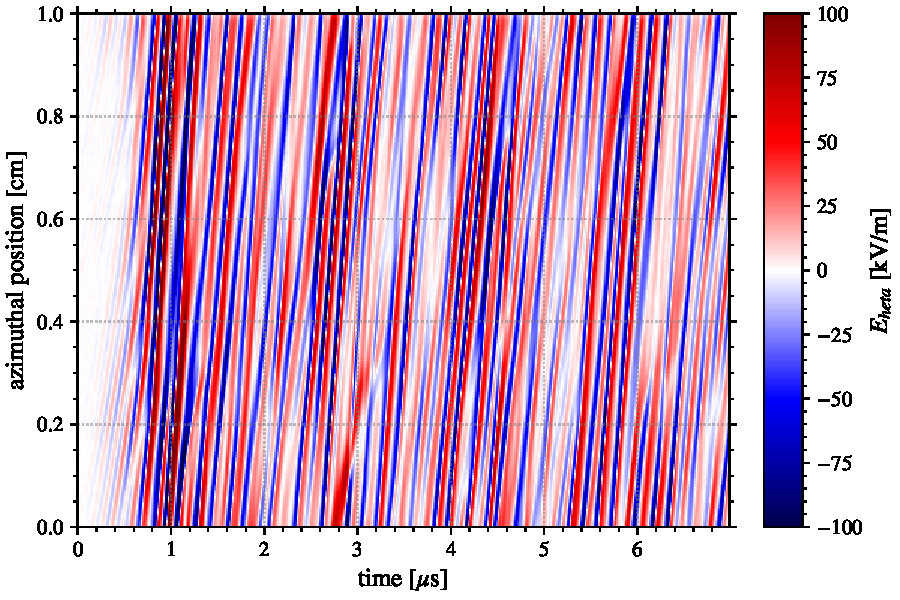
\includegraphics[width=\defaultwidth]{electric_field_cut2D}
    \caption{Temporal evolution of the azimuthal electric field as a function of the azimuthal position.}
    \label{fig-2DcutEx}
  \end{figure}

  \Cref{fig-FFT_ex} shows the frequency spectrum of the azimuthal electric field presented in \cref{fig-2DcutEx} computed via \ac{FFT} in the stationary state ($t > 1.2\,\micro\second$).
  The spectrum have been averaged in the azimuthal direction, in order to reduce the noise.
  The theoretical frequency $f_{\rm theo} = \frac{\opi}{\pi \sqrt{6} }$ is given \citep{croes2018}. 
  We can see a very good agreement between $f_{\rm theo}$ and the maximum of the frequency spectrum.
  \begin{figure}[hbt]
    \centering
    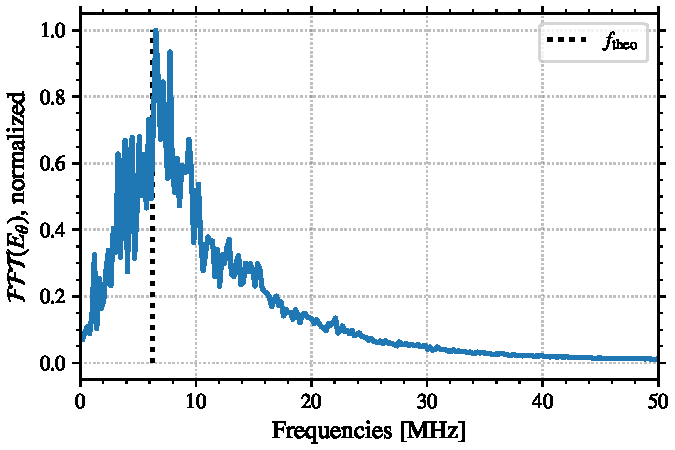
\includegraphics[width=\defaultwidth]{spectrum_frequency}
    \caption{Frequency spectrum of the azimuthal electric field, averaged in the azimuthal direction. The black line is the theoretical frequency.}
    \label{fig-FFT_ex}
  \end{figure}
  
  \subsection{Energy cascade} \label{subsec-turbul}
  
  We can see in \cref{fig-FFT_ex} a slow decrease of the frequency amplitude from $f_{\rm theo}$ to larger frequencies.
  This sort of cascade is typical of turbulences, and can be a source of energy dissipation hence saturation.
  Kolmogorov's hypothesis of incompressible fluid leads to a cascade in power law \[ W(f) = | \mathcal{FFT}(E_{\theta})(f) |^2 \propto f ^ {- \alpha}, \]
  with $\alpha = 5/3$.
  
  \begin{figure}[hbt]
    \centering
    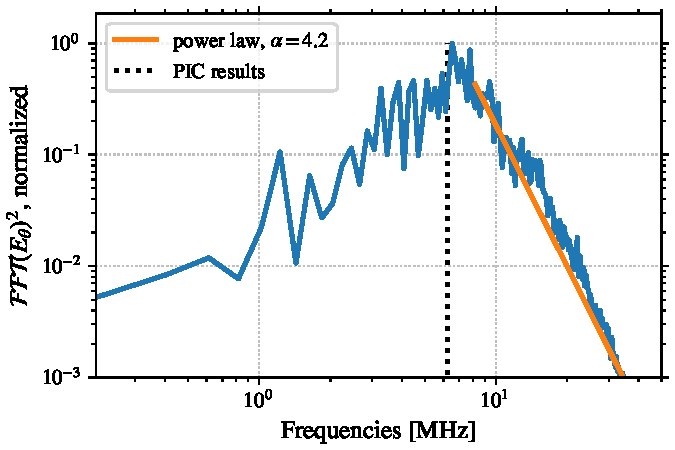
\includegraphics[width=\defaultwidth]{spectrum_frequency_turbul}
    \caption{Frequency power spectrum, normalized and in log-log scale. }
    \label{fig-turbul}
  \end{figure}
  
  \Cref{fig-turbul} shows the frequency power spectrum in log scale.
  Is overlaid a fit of the cascade, for frequencies above the maximum amplitude.
  The power law obtained is $\alpha \simeq 4.2$.
  The oscillations observed present a decrease of the power spectrum much steeper than expected from turbulences.
  Even if the mechanism of plasma turbulences differs from the fluid \citep{tsytovich1972}, the value of $\alpha$ is quite large, hence we dismiss this phenomenon.
  
  \subsection{Temporal evolution of the oscillation amplitude} \label{subsec-temp}
  We have seen in the previous section that after a growing phase, the instability saturates while oscillates slowly around the stable value.
  This section analyses these temporal characteristics.
  
  \Cref{fig-Ezstd_time} shows the temporal evolution of the characteristics of the electrostatic oscillation.
  As the oscillation is not monochromatic (i.e. it is the sum of multiple waves), we display both the maximum of the electric field $\max(E_{\theta})$, and its standard deviation $\stdE$.
  In the case of a monochromatic wave, one would have 
  \[ \stdE = \frac{\max(E_{\theta})}{\sqrt{2}}.  \]
  
  \begin{figure}[hbt]
    \centering
    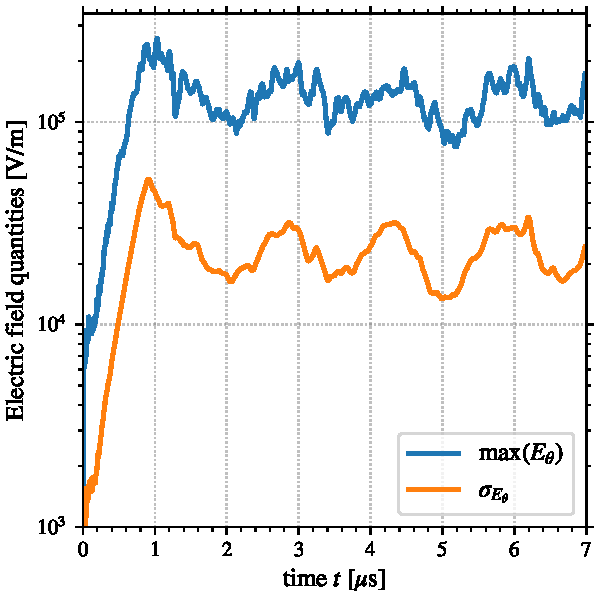
\includegraphics[width=\defaultwidth]{Temporal_E_theta.pdf}
    \caption{Temporal evolution of the maximum and the standard deviation of the azimuthal electric field, in log scale.}
    \label{fig-Ezstd_time}
  \end{figure}
  
  We can see in \cref{fig-Ezstd_time} that during the first microsecond, we observe an exponential growth, corresponding to a constant growth rate.
  A linear fit in log scale give $\gamma_{PIC} \simeq 0.07 \opi$ during the linear phase.
  After $t=1\,\micro\second$, the amplitude of the electric field oscillates around a mean value, with a period of the order of $T_{NL}=1.5 \pm 0.1 \,\micro\second$.
  Hence, the azimuthal electric field becomes of the type of
  \[  E_{\theta} = E_{\rm LF}(t) E_{\rm HF}(t, {\theta}) \]
  with $E_{\rm HF}(t) $ the high frequency instability, and $E_{\rm LF}(t)$ the modulation of low frequency $f_{\rm LF} \simeq  650 \pm 40 \,\kilo\hertz$.
  Several phenomena are candidates to the modulation observed.
  they are discussed here-after.
  
  
  \paragraph{Ion transit time\\}
    The ions are injected at the anode, and are accelerated by the uniform axial electric field $E_z$.
    The transit time of the ions in the axial direction $T_t$  is the time needed for the ions to travel $L_z$
    \begin{equation} \label{eq-transittime}
      T_{t} = \sqrt{\frac{2 m_i L_z}{e E_z}} \simeq 0.8 \mu s.
    \end{equation}
    
    The transit time is of the good  order of magnitude, but $T_{NL}$ is still twice bigger.
    
  \paragraph{Particle trapping and bouncing\\}
    A common reason for wave saturation is the ion trapping. 
    It has been observed in both \ac{1D} simulation by \citet{lafleur2016a} and in \ac{2D} simulation \citep{croes2017a}.
    Hence, the low frequency modulation could be due to particle bouncing \citep{belmont2013}.
    However, the bouncing time scale is 
    \begin{equation} \label{eq-TB}
      T_{B} = 2 \pi \sqrt{\frac{m_i}{e k \max(E_{\theta})} } \simeq 0.5 \,\micro\second,
    \end{equation}
    which is 3 times smaller than $T_{NL}$.
    Using $\sqrt{2} \sigma_{E_{\theta}}$ instead of $\max(E)$, we find $T_B = 0.9\,\micro\second$
    Even though in \citet{belmont2013}, the authors say that, when the amplitude of the electric field is large (as it is the case here), the bouncing time scale increases due to non-linear phenomenon (the particle trajectory is no longer harmonic), we cannot conclude here that this is the origin of the low frequency modulation.

  
  \paragraph{Ion trapping oscillation\\}
    The wave saturating due to ion trapping has an amplitude of \citep{boeuf2018}
     \begin{equation} \label{eq-iontropempl}
       \stdE \leq \frac{\Te}{12 \lde}.
     \end{equation}
    
    Defining the wave energy  density by
    \begin{equation} \label{eq-waveE}
      \epsilon_{\rm wave} = \frac{\epsilon_0}{2} \stdE^2
    \end{equation}
    and the electron thermal energy density with
    \begin{equation} \label{eq-thE}
      \epsilon_{\rm th} = \frac{3}{2} e n_e \Te
    \end{equation}
    
    We find the criteria for the ion trapping
    \begin{equation} \label{eq-criteriaIT}
      432 \epsilon_{\rm wave} \leq \epsilon_{\rm th}.
    \end{equation}
    
    \Cref{fig-tempITcrit} shows the temporal evolution of the electron thermal energy $\epsilon_{\rm th}$ and the wave energy density $\epsilon_{\rm wave}$, scaled by the factor 432.
    We can see that $\epsilon_{\rm th}$ is relatively constant.
    However, $\epsilon_{\rm wave}$  oscillates significantly, and passes regularly above and below $\epsilon_{\rm th}$.
    
    \begin{figure}[hbt]
      \centering
      % 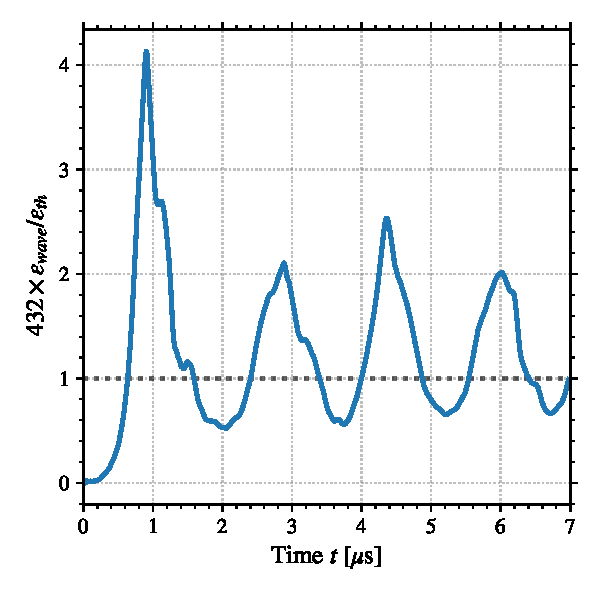
\includegraphics[width=\defaultwidth]{Ion_Trapping_criter}
      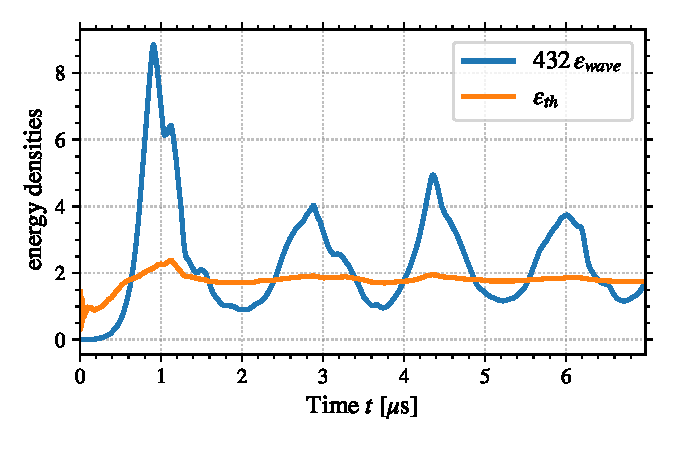
\includegraphics[width=\defaultwidth]{Ion_Trapping_criter_bis}
      \caption{Temporal evolution of the wave energy density (scaled) compared to the thermal energy density.}
      \label{fig-tempITcrit}
    \end{figure}
    
    In \cref{fig-tempITcrit}, as expected the period of the oscillations of $\epsilon_{\rm wave}$ is $T_{NL} = 1.5\,\micro\second$.
    But here, we can see that when the criterion \cref{eq-criteriaIT} is fulfilled, the temporal derivative of the growth rate is positive.
    However, a delay $\tau$ after the moment when the criteria is violated ($\tau = 0.40 \pm 0.07 \,\micro\second$ on the four oscillations), the wave abruptly stops rising and decreases instead.
    This delay between the time the ions should be trapped and the time the wave stops growing in most certainly due to the ion inertia, as we have $\tau \sim T_B$.
    
    Complementary results are presented in \cref{subsec-VDFIAW} by solving the dispersion relations.
    
